% !TeX program = xelatex
\documentclass[aspectratio=169,17pt,fleqn]{beamer}

\usetheme{Madrid}
\usecolortheme{dolphin}
\setbeamertemplate{navigation symbols}{}
\setbeamertemplate{footline}[frame number]

% --- Fonts ---
\usepackage{fontspec}      % text fonts (beamer uses sans by default)
\usepackage{unicode-math}  % modern math
% Alternatives:
% \setmathfont{XITS Math}
% \setmathfont{TeX Gyre Pagella Math}

% --- Math packages (keep these) ---
\usepackage{amsmath,mathtools}
% \usepackage{amssymb} % <-- REMOVE this when using unicode-math

\usepackage{booktabs,array}
\usepackage{tikz}
\usetikzlibrary{tikzmark,positioning,fit,calc,arrows.meta}

% ... (rest of your preamble unchanged)

% MACROS
\newcommand{\seq}{\vdash}
\newcommand{\A}{\mathrm{A}}

\AtBeginSection[]{
  \begin{frame}
    \centering
    \vfill
    \Large\insertsectionhead
    \vfill
  \end{frame}
}

\title{Week 7}
\author{Hans Halvorson}
\institute{Princeton University}
\date{October 20, 2025}

\begin{document}


% Enter presentation title:
\title{Lecture 7: Invitation to Predicate Logic}
% Enter presentation information:
\frame{\titlepage}

% Fill out content of presentation:
\begin{frame}
  \frametitle{Overview}

  
\begin{enumerate}
\item Motivation: Propositional logic cannot see all logical relations
\item A more fine-grained grammar
  \begin{itemize}
  \item Names and predicates
  \item Variables and quantifiers
  \end{itemize}
\item Translation
\item Inference rules
  \begin{itemize}
  \item $\forall$ elimination
  \item $\forall$ introduction
  \end{itemize}
\end{enumerate}
\end{frame}


\section{Propositional logic is inadequate}

\begin{frame}{Validities that escape propositional logic}

  \begin{itemize}
  \item All people are mortal.
  \item Socrates is a person.
  \item Therefore, Socrates is mortal.
  \end{itemize}

\vspace{2em}

If the subject and predicate of sentences are not both the same, then
propositional logic does not recognize any relation between them.

\end{frame}


% In your preamble:
% \usepackage{tikz,xcolor}
% \usetikzlibrary{positioning}

\definecolor{whale}{RGB}{52,120,220}
\definecolor{mammal}{RGB}{255,130,0}
\definecolor{lung}{RGB}{0,160,80}

\begin{frame}[t]{Validities that escape propositional logic}

\begin{columns}[T,onlytextwidth]
\column{0.55\textwidth}
\begin{itemize}
  \item All \textcolor{whale}{\textbf{whales}} are \textcolor{mammal}{\textbf{mammals}}.
  \item All \textcolor{mammal}{\textbf{mammals}} have \textcolor{lung}{\textbf{lungs}}.
  \item Therefore: All \textcolor{whale}{\textbf{whales}} have
    \textcolor{lung}{\textbf{lungs}}.
\end{itemize}

\bigskip
\[
  \mathsf{All}(\textcolor{whale}{W},\textcolor{mammal}{M}),
  \mathsf{All}(\textcolor{mammal}{M},\textcolor{lung}{L}) \:\vdash\:
  \mathsf{All}(\textcolor{whale}{W},\textcolor{lung}{L})
\]

\column{0.45\textwidth}
\begin{tikzpicture}[scale=1.1, every node/.style={font=\small}]
  % nested circles (Barbara: S⊆M⊆P)
  \fill[lung!20] (0,0) circle (1.8);
  \fill[mammal!25] (0,0) circle (1.3);
  \fill[whale!30] (0,0) circle (0.8);

  \draw[thick,lung!70!black] (0,0) circle (1.8);
  \draw[thick,mammal!80!black] (0,0) circle (1.3);
  \draw[thick,whale!80!black] (0,0) circle (0.8);

  \node[lung!60!black] at (1.3,1.3) {lung-havers};
  \node[mammal!80!black] at (0.9,0.6) {mammals};
  \node[whale!80!black] at (0.5,0.05) {whales};
\end{tikzpicture}
\end{columns}

\end{frame}


\begin{frame}{When propositional logic falls short}

\begin{block}{Example from mathematics}
If a number is even, its square is even.  
$4$ is even.  
\hfill$\therefore$ $4^2$ is even.
\end{block}

\begin{columns}[T,onlytextwidth]
  \column{0.35\textwidth}
  \small 
\textbf{Propositional view:}

$ P, P\to Q \:\vdash\:Q $ 


\column{0.65\textwidth}
\small 
\textbf{Mathematical structure:}

$\forall n\, (E(n)\to E(n^2)), E(4)\: \vdash\: E(4^2)$

\end{columns}

\end{frame}


\begin{frame}{Diagnosis}

  \begin{itemize}
  \item The inadequacy of propositional logic cannot be fixed by
    adding more inference rules.
    \begin{itemize}
      \item If we add any additional rules, then our system would
        become inconsistent.
     \end{itemize}
   \item Have we missed some propositional connectives?
     \begin{itemize}
  \item No, there is a precise sense in which our set of connectives
    is \textbf{conceptually complete}. \end{itemize}
\end{itemize}

\end{frame}

\begin{frame}{The predicate calculus}

  \begin{itemize}
  \item In the early 20th century, the missing logical structure was
    identified, represented symbolically, and codified in a
    ``calculus''.
  \end{itemize}


\end{frame}

\section{Sub-propositional grammar}

\begin{frame}[t]{Names and predicates}

\begin{flushleft}
Alice is French.

\vspace{3em}

Bernard is French.

\vspace{3em}

Alice is German.
\end{flushleft}

\vfill
\end{frame}

%%

\begin{frame}{Quantified sentences}

  \begin{itemize}
  \item You are familiar with the concept of a variable from
    mathematics.
  \item Natural languages do not explicitly use variables.
  \item Hypothesis: ``All'' and ``Some'' sentences are best
    analyzed as consisting of predicate symbols, variables, and
    quantifiers. \end{itemize}

\end{frame}  

\begin{frame}{Variables}

\begin{tabular}{l@{\hspace{4em}}l}  
  Alice is French. & $Fa$ \\[1em]
  $x$ is French. & $Fx$ \\[1em]
  Someone is French. & ? \\[1em]
 There is an $x$ such that $x$ is French. & $\exists xFx$ \end{tabular}


\end{frame}

\begin{frame}{Formulas}

  \begin{itemize}
  \item We don't call ``$Fx$'' a proposition, since it cannot be true
    or false.
  \item We call ``$Fx$'' a \textbf{formula}.
  \item Adding the quantifier ``$\exists x$'' to ``$Fx$'' creates a
    sentence.
  \end{itemize}

\end{frame}

\begin{frame}{Universal quantifier}

\begin{tabular}{@{}p{0.7\textwidth}l@{}}
All whales are mammals. &
? \\[1.5ex]

If $a$ is a whale then $a$ is a mammal. &
$W a \to M a$ \\[1.5ex]

For any $x$, if $x$ is a whale then $x$ is a mammal. &
$\forall x (W x \to M x)$ \\
\end{tabular}

\end{frame}

\begin{frame}[t]{Standard syllogistic forms}

\medskip 
\setlength{\tabcolsep}{0pt} % tighter edges
\begin{tabular}{@{}p{0.68\textwidth}p{0.31\textwidth}@{}}
\textbf{All Finns are gregarious.}              & $\forall x\,\big(Fx \to Gx\big)$ \\[1.2em]
\textbf{Some Finns are gregarious.}             & $\exists x\,\big(Fx \wedge Gx\big)$ \\[1.2em]
\textbf{No Finns are gregarious.}               & $\forall x\,\big(Fx \to \neg Gx\big)$ \\[1.2em]
% (equivalently: $\neg \exists x\,(Fx \wedge Gx)$)
\textbf{Some Finns are not gregarious.}         & $\exists x\,\big(Fx \wedge \neg Gx\big)$ \\
\end{tabular}

\end{frame}


\begin{frame}

  \medskip 

  All happy Finns are gregarious.

  \vspace{3em}

  All Finns and Germans are happy.

  \vspace{3em}

\end{frame}

\begin{frame}

  \vfill

  No dogs or cats are permitted in the restaurant.

  \vfill 


\end{frame}

\begin{frame}

  $\forall x(Fx\to P)$

  \hspace{1.5em} Everything has the feature that if it is $F$, then $P$
  holds.

  \bigskip

  $\forall xFx\to P$

  \hspace{1.5em} If everything has the feature $F$, then $P$ holds.


\end{frame}

\begin{frame}{Relations}

  Maren is taller than Niels.
  \vspace{1.5em}

  Maren is taller than someone.

  \vspace{1.5em}

  Someone is taller than Niels.

  \vspace{1.5em}

\end{frame}

\begin{frame}

  Everyone is taller than someone.
  \vspace{1.5em}

  Someone is taller than everyone.
  \vspace{1.5em}

\end{frame}

\begin{frame}

  There is a student who admires every professor.
  \[ \exists x(Sx\wedge \forall y(Py\to Axy)) \]

  There is a professor whom every student admires.
  \[ \exists x(Px\wedge \forall y(Sy\to Ayx)) \]

  Every student admires some professor.
  \[ \forall x(Sx\to \exists y(Py\wedge Axy)) \]
  
\end{frame}


\section{Inference to/from quantified statements}

\begin{frame}{$\forall$ elimination}

  The idea behind $\forall$ elimination is straightforward:

  \medskip From a universal statement, any \textbf{instance} follows
  logically.

  \[ \begin{array}{c}
       \forall x\,\varphi (x) \\ \hline
       \varphi (a) \end{array} \]



\end{frame}
\begin{frame}{$\forall$ elimination}

  $\forall x(Fx\to Gx),Fa \:\vdash\: Ga $

  \bigskip \begin{tabular}{>{\raggedleft\arraybackslash}p{1.5cm} >{\centering\arraybackslash}p{1.0cm} p{5cm} >{\raggedright\arraybackslash}p{3.5cm}}
1 & (1) & $\forall x (Fx \to Gx)$ & A \\
2 & (2) & $Fa$ & A \\
1 & (3) & $Fa \to Ga$ & 1 UE \\
1,2 & (4) & $Ga$ & 3,2 MP \\
\end{tabular}

\end{frame}

\begin{frame}
  $\forall x\forall y(Fx\wedge Gy)\:\vdash\: Fa\wedge Gb$

  \bigskip \begin{tabular}{>{\raggedleft\arraybackslash}p{1.5cm} >{\centering\arraybackslash}p{1.0cm} p{5cm} >{\raggedright\arraybackslash}p{3.5cm}}
1 & (1) & $\forall x \forall y (Fx \wedge Gy)$ & A \\
1 & (2) & $\forall y (Fa \wedge Gy)$ & 1 UE \\
1 & (3) & $Fa \wedge Gb$ & 2 UE \\
\end{tabular}


\end{frame}

\begin{frame}
  $\forall x\forall y(Fx\wedge Gy)\:\vdash\: Fa\wedge Ga$

    \bigskip \begin{tabular}{>{\raggedleft\arraybackslash}p{1.5cm} >{\centering\arraybackslash}p{1.0cm} p{5cm} >{\raggedright\arraybackslash}p{3.5cm}}
1 & (1) & $\forall x \forall y (Fx \wedge Gy)$ & A \\
1 & (2) & $\forall y (Fa \wedge Gy)$ & 1 UE \\
1 & (3) & $Fa \wedge Ga$ & 2 UE \\
\end{tabular}


  
\end{frame}

\begin{frame}
  $P\to\forall xFx \:\vdash\: P\to Fa$

  \bigskip \begin{tabular}{>{\raggedleft\arraybackslash}p{1.5cm} >{\centering\arraybackslash}p{1.0cm} p{5cm} >{\raggedright\arraybackslash}p{3.5cm}}
1 & (1) & $P \to \forall x Fx$ & A \\
2 & (2) & $P$ & A \\
1,2 & (3) & $\forall x Fx$ & 1,2 MP \\
1,2 & (4) & $Fa$ & 3 UE \\
1 & (5) & $P \to Fa$ & 2,4 CP \\
\end{tabular}


\end{frame}

\begin{frame}
  $\neg Fa\vdash \neg\forall xFx$

  \bigskip \begin{tabular}{>{\raggedleft\arraybackslash}p{1.5cm} >{\centering\arraybackslash}p{1.0cm} p{5cm} >{\raggedright\arraybackslash}p{3.5cm}}
1 & (1) & $\neg Fa$ & A \\
2 & (2) & $\forall x Fx$ & A \\
2 & (3) & $Fa$ & 2 UE \\
1,2 & (4) & $Fa \wedge \neg Fa$ & 3,1 $\wedge$I \\
1 & (5) & $\neg \forall x Fx$ & 2,4 RA \\
\end{tabular}


\end{frame}  

\begin{frame}{Warnings}

  Only apply UE when the entire sentence on the line is
  universally quantified. 
  
  \bigskip $\forall x(Fx\to P)$ \\
  $\forall x(Fx\to \forall yGy)$ \\
  $\forall xFx\to Ga$ \\
  $\forall x\forall yRxy$
  

\end{frame}

\begin{frame}{Warnings}

  When applying UE, replace all instances of the relevant variable
  with the same name.

  \bigskip $\forall x(Fx\to \forall yRxy)$



\end{frame}


\begin{frame}{From one individual to everyone}

\begin{block}{Intuitive idea}
To show that \textbf{everyone} has a property,  
we can reason about \textbf{one individual chosen at random}.
\end{block}

\medskip

\begin{columns}[T,onlytextwidth]
\column{0.58\textwidth}
\begin{itemize}
  \item Suppose we want to prove that all whales have lungs.
  \item We pick a whale—call it $a$.
  \item We reason about $a$ as if it were any whale.
\end{itemize}

\column{0.42\textwidth}
\centering
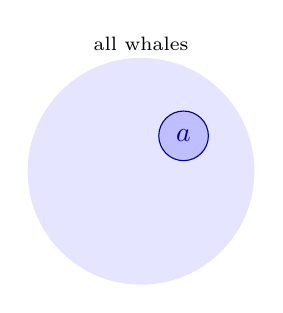
\begin{tikzpicture}[scale=0.9]
  \fill[blue!10] (0,0) circle (1.6);
  \node at (0,1.8) {\scriptsize all whales};
  \filldraw[blue!60!black,fill=blue!25] (0.6,0.5) circle (0.35);
  \node[blue!60!black] at (0.6,0.5) {$a$};
\end{tikzpicture}
\end{columns}
\end{frame}


\begin{frame}{What does it mean for $a$ to be \emph{arbitrary}?}

\begin{block}{Arbitrary name}
The name $a$ is \textbf{arbitrary} when nothing in the proof
depends on any \emph{special feature} of $a$.
\end{block}

\medskip
\begin{itemize}
  \item Our reasoning about $a$ must not rely on  
        facts like “$a$ lives in the Pacific” or “$a$ is the largest whale.”
  \item The argument must hold no matter which whale we picked.
\end{itemize}

\bigskip
\centering
\textit{An arbitrary name stands for an individual we reason about generally.}

\end{frame}

\begin{frame}{From arbitrariness to universal generalization}

\begin{block}{Bridge to Universal Introduction}
If we can prove $\varphi(a)$ using $a$ as an \textbf{arbitrary name},  
then we may infer the general statement $\forall x\,\varphi(x)$.
\end{block}

\medskip
\[
\frac{\ \varphi(a)\ }{\ \forall x\,\varphi(x)\ }\text{UI}
\quad
\text{\small(side condition: $a$ not free in any open assumption)}
\]

\bigskip
\begin{itemize}
  \item The conclusion applies to \emph{all} objects of that kind.  
  \item The key is that $a$ never referred to anything special.  
\end{itemize}

\end{frame}

\begin{frame}{Universal introduction}

  From a line
  
  \medskip \begin{tabular}{l l l l}
    $\Gamma$ & (m) & $\varphi (a)$ \end{tabular}

  \medskip  we may infer

  \medskip \begin{tabular}{l l l l}
    $\Gamma$ & (n) & $\forall x\,\varphi (x)$  \end{tabular}
  
  \medskip provided that the name ``$a$'' does not occur in any of the
  sentences listed in $\Gamma$ or in $\varphi (x)$.




\end{frame}






\begin{frame}
  \frametitle{$\forall$ introduction}

  $\forall x(Fx\to Gx),\forall xFx \:\vdash\: \forall xGx$

  \bigskip \begin{tabular}{>{\raggedleft\arraybackslash}p{1.5cm} >{\centering\arraybackslash}p{1.0cm} p{5cm} >{\raggedright\arraybackslash}p{3.5cm}}
1 & (1) & $\forall x (Fx \to Gx)$ & A \\
2 & (2) & $\forall x Fx$ & A \\
2 & (3) & $Fa$ & 2 UE \\
1 & (4) & $Fa\to Ga$ & 1 UE \\
1,2 & (5) & $Ga$ & 4,3 MP \\
1,2 & (6) & $\forall x Gx$ & 5 UI \\
\end{tabular}


\end{frame}

\begin{frame}

  $\vdash\:\forall x(Fx\to (Fx\vee Gx))$

  \bigskip \begin{tabular}{>{\raggedleft\arraybackslash}p{1.5cm} >{\centering\arraybackslash}p{1.0cm} p{6.5cm} >{\raggedright\arraybackslash}p{3.5cm}}
1 & (1) & $Fa$ & A \\
1 & (2) & $Fa\vee Ga$ & 1 $\vee$I \\
$\varnothing$ & (3) & $Fa\to (Fa\vee Ga)$ & 1,2 CP \\
$\varnothing$ & (4) & $\forall x (Fx\to (Fx\vee Gx))$ & 3 UI \\
\end{tabular}


\end{frame}

\begin{frame}

  $\forall x(P\to Fx)\:\vdash \:P\to \forall xFx$

  \bigskip \begin{tabular}{>{\raggedleft\arraybackslash}p{1.5cm} >{\centering\arraybackslash}p{1.0cm} p{5cm} >{\raggedright\arraybackslash}p{3.5cm}}
1 & (1) & $\forall x (P \to Fx)$ & A \\
2 & (2) & $P$ & A \\
1 & (3) & $P \to Fa$ & 1 UE \\
1,2 & (4) & $Fa$ & 3,2 MP \\
1,2 & (5) & $\forall x Fx$ & 4 UI \\
1 & (6) & $P \to \forall x Fx$ & 2,5 CP \\
\end{tabular}

  

\end{frame}

\begin{frame}

  $P\to \forall xFx\:\vdash\: \forall x(P\to Fx)$

  \bigskip \begin{tabular}{>{\raggedleft\arraybackslash}p{1.5cm} >{\centering\arraybackslash}p{1.0cm} p{5cm} >{\raggedright\arraybackslash}p{3.5cm}}
1 & (1) & $P \to \forall x Fx$ & A \\
2 & (2) & $P$ & A \\
1,2 & (3) & $\forall x Fx$ & 1,2 MP \\
1,2 & (4) & $Fa$ & 3 UE \\
1 & (5) & $P \to Fa$ & 2,4 CP \\
1 & (6) & $\forall x (P \to Fx)$ & 5 UI \\
\end{tabular}



\end{frame}

\begin{frame}{Precisifying the UI rule}

  $\forall$I requires replacing \textbf{all} instances of the
  arbitrary name.

  \bigskip \begin{tabular}{>{\raggedleft\arraybackslash}p{1.5cm}
             >{\centering\arraybackslash}p{1.0cm} p{6cm}
             >{\raggedright\arraybackslash}p{3.5cm} p{3cm}}
             1 & (1) & $\forall xRxx$ & A \\
             1 & (2) & $Raa$ & 1 UE \\
             1 & (3) & $\forall xRxa$ & 2 UI & error!\\
             1 & (4) & $\forall y\forall xRxy$ & 3 UI \end{tabular}

\end{frame}           

\begin{frame}{Precisifying the UE rule}

  But UE does allow instantiating to a name that already occurs in the
  formula.

  \bigskip \begin{tabular}{>{\raggedleft\arraybackslash}p{1.5cm} >{\centering\arraybackslash}p{1.0cm} p{5cm} >{\raggedright\arraybackslash}p{3.5cm}}
             1 & (1) & $\forall x\forall yRxy$ & A \\
             1 & (2) & $\forall yRay$ & 1 UE \\
             1 & (3) & $Raa$          & 2 UE \\
             1 & (4) & $\forall xRxx$ & 3 UI \end{tabular}

\end{frame}

\begin{frame}{Precisifying the UE rule}

UE allows us to choose any name --- same or different from what
already occurs.           

      \bigskip \begin{tabular}{>{\raggedleft\arraybackslash}p{1.5cm}
      >{\centering\arraybackslash}p{1.0cm} 
      >{\raggedright\arraybackslash}p{6cm} p{3cm}}
                                   1 & (1) & $\forall x\forall yRxy$ & A \\
                      1 & (2) & $\forall yRay$ & 1 UE \\
                      1 & (3) & $Rab$ & 2 UE \\
                      1 & (4) & $\forall xRxb$ & 3 UI \\
                      1 & (5) & $\forall y\forall xRxy$ & 4 UI \end{tabular}
           


\end{frame}  

       


\end{document}
%%% Local Variables:
%%% TeX-engine: xetex
%%% TeX-master: t
%%% End:
